\section{Results}

\subsection*{Other Capabilities}

We produced a highly accessible CAD program suitable for laser cutting. The accessibility of 2to3D can be attributed to the fact that the program runs entirely in the browser (thus requiring no additional software beyond a modern browser), and that the program strips away all non-essential drawing features and all 3D modeling features. Currently 2to3D only supports the creation of drawings intended for translation into cutting paths. Figure~\ref{fig:usingProgram} depicts a full digital fabrication workflow using 2to3D. The figure depicts the design of a press-fit box. The laser cutter available for use utilized CorelDRAW for CAM so the drawing was exported from 2to3D as a SVG and imported to CorelDRAW for printing.

\begin{figure}[H]
  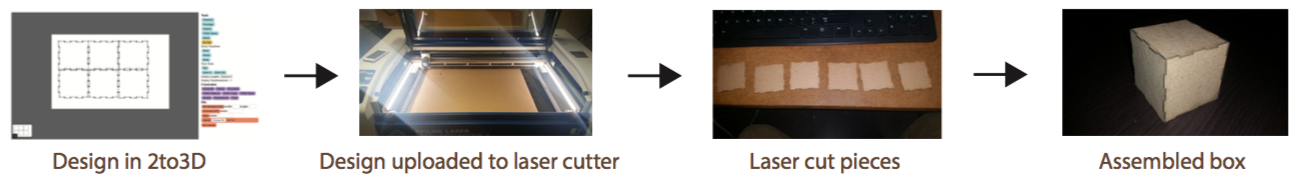
\includegraphics[width=\linewidth]{usingProgram.jpg}
  \caption{Full digital fabrication workflow using 2to3D. The laser cutter we had access to used CorelDraw for CAM so the drawing was created in 2to3D and imported to CorelDraw just for printing.}
  \label{fig:usingProgram}
\end{figure}

2to3D has a simple design that displays all tools to the user without being overwhelming. This design inspired by ``lean-operating practices" also immediately and constantly conveys program state information by highlighting the current tool and changing the cursor style. Figures \ref{fig:screenshot} and \ref{fig:screenshot2} are screenshots of the program.

\begin{figure}[H]
  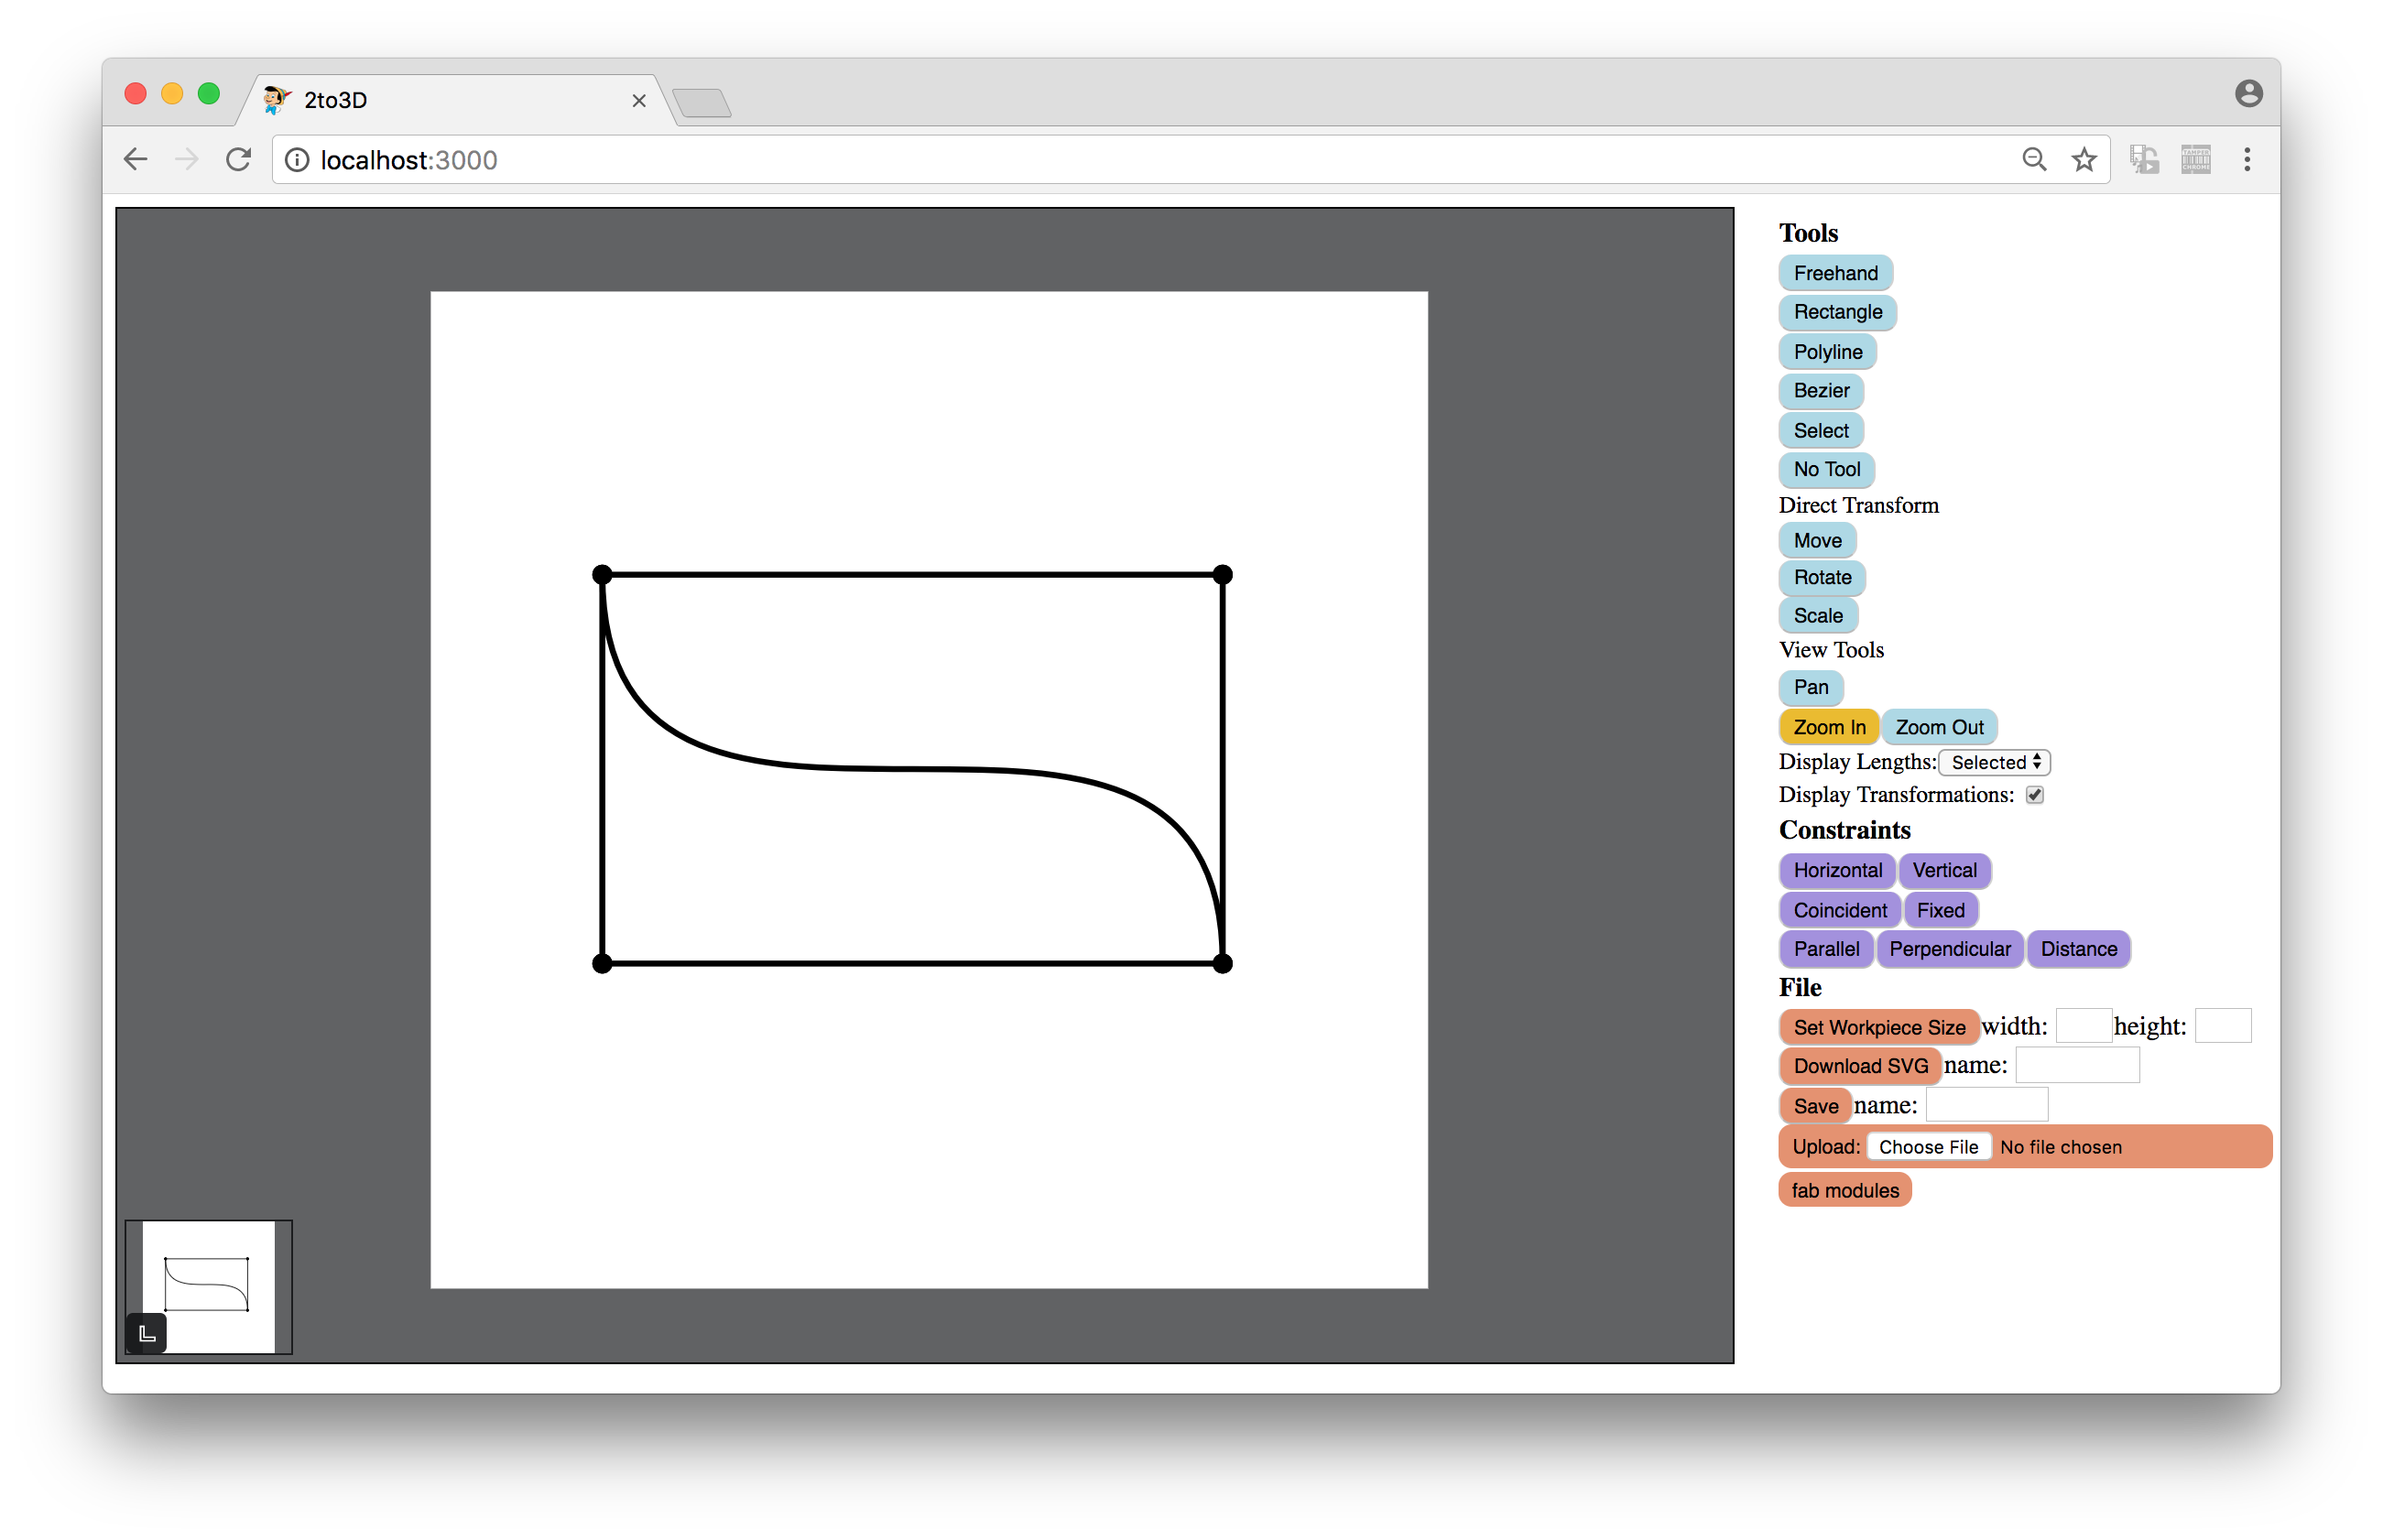
\includegraphics[width=\linewidth]{screenshot.png}
  \caption{Screenshot of 2to3D program depicting example bezier and rectangle.}
  \label{fig:screenshot}
\end{figure}

\begin{figure}[H]
  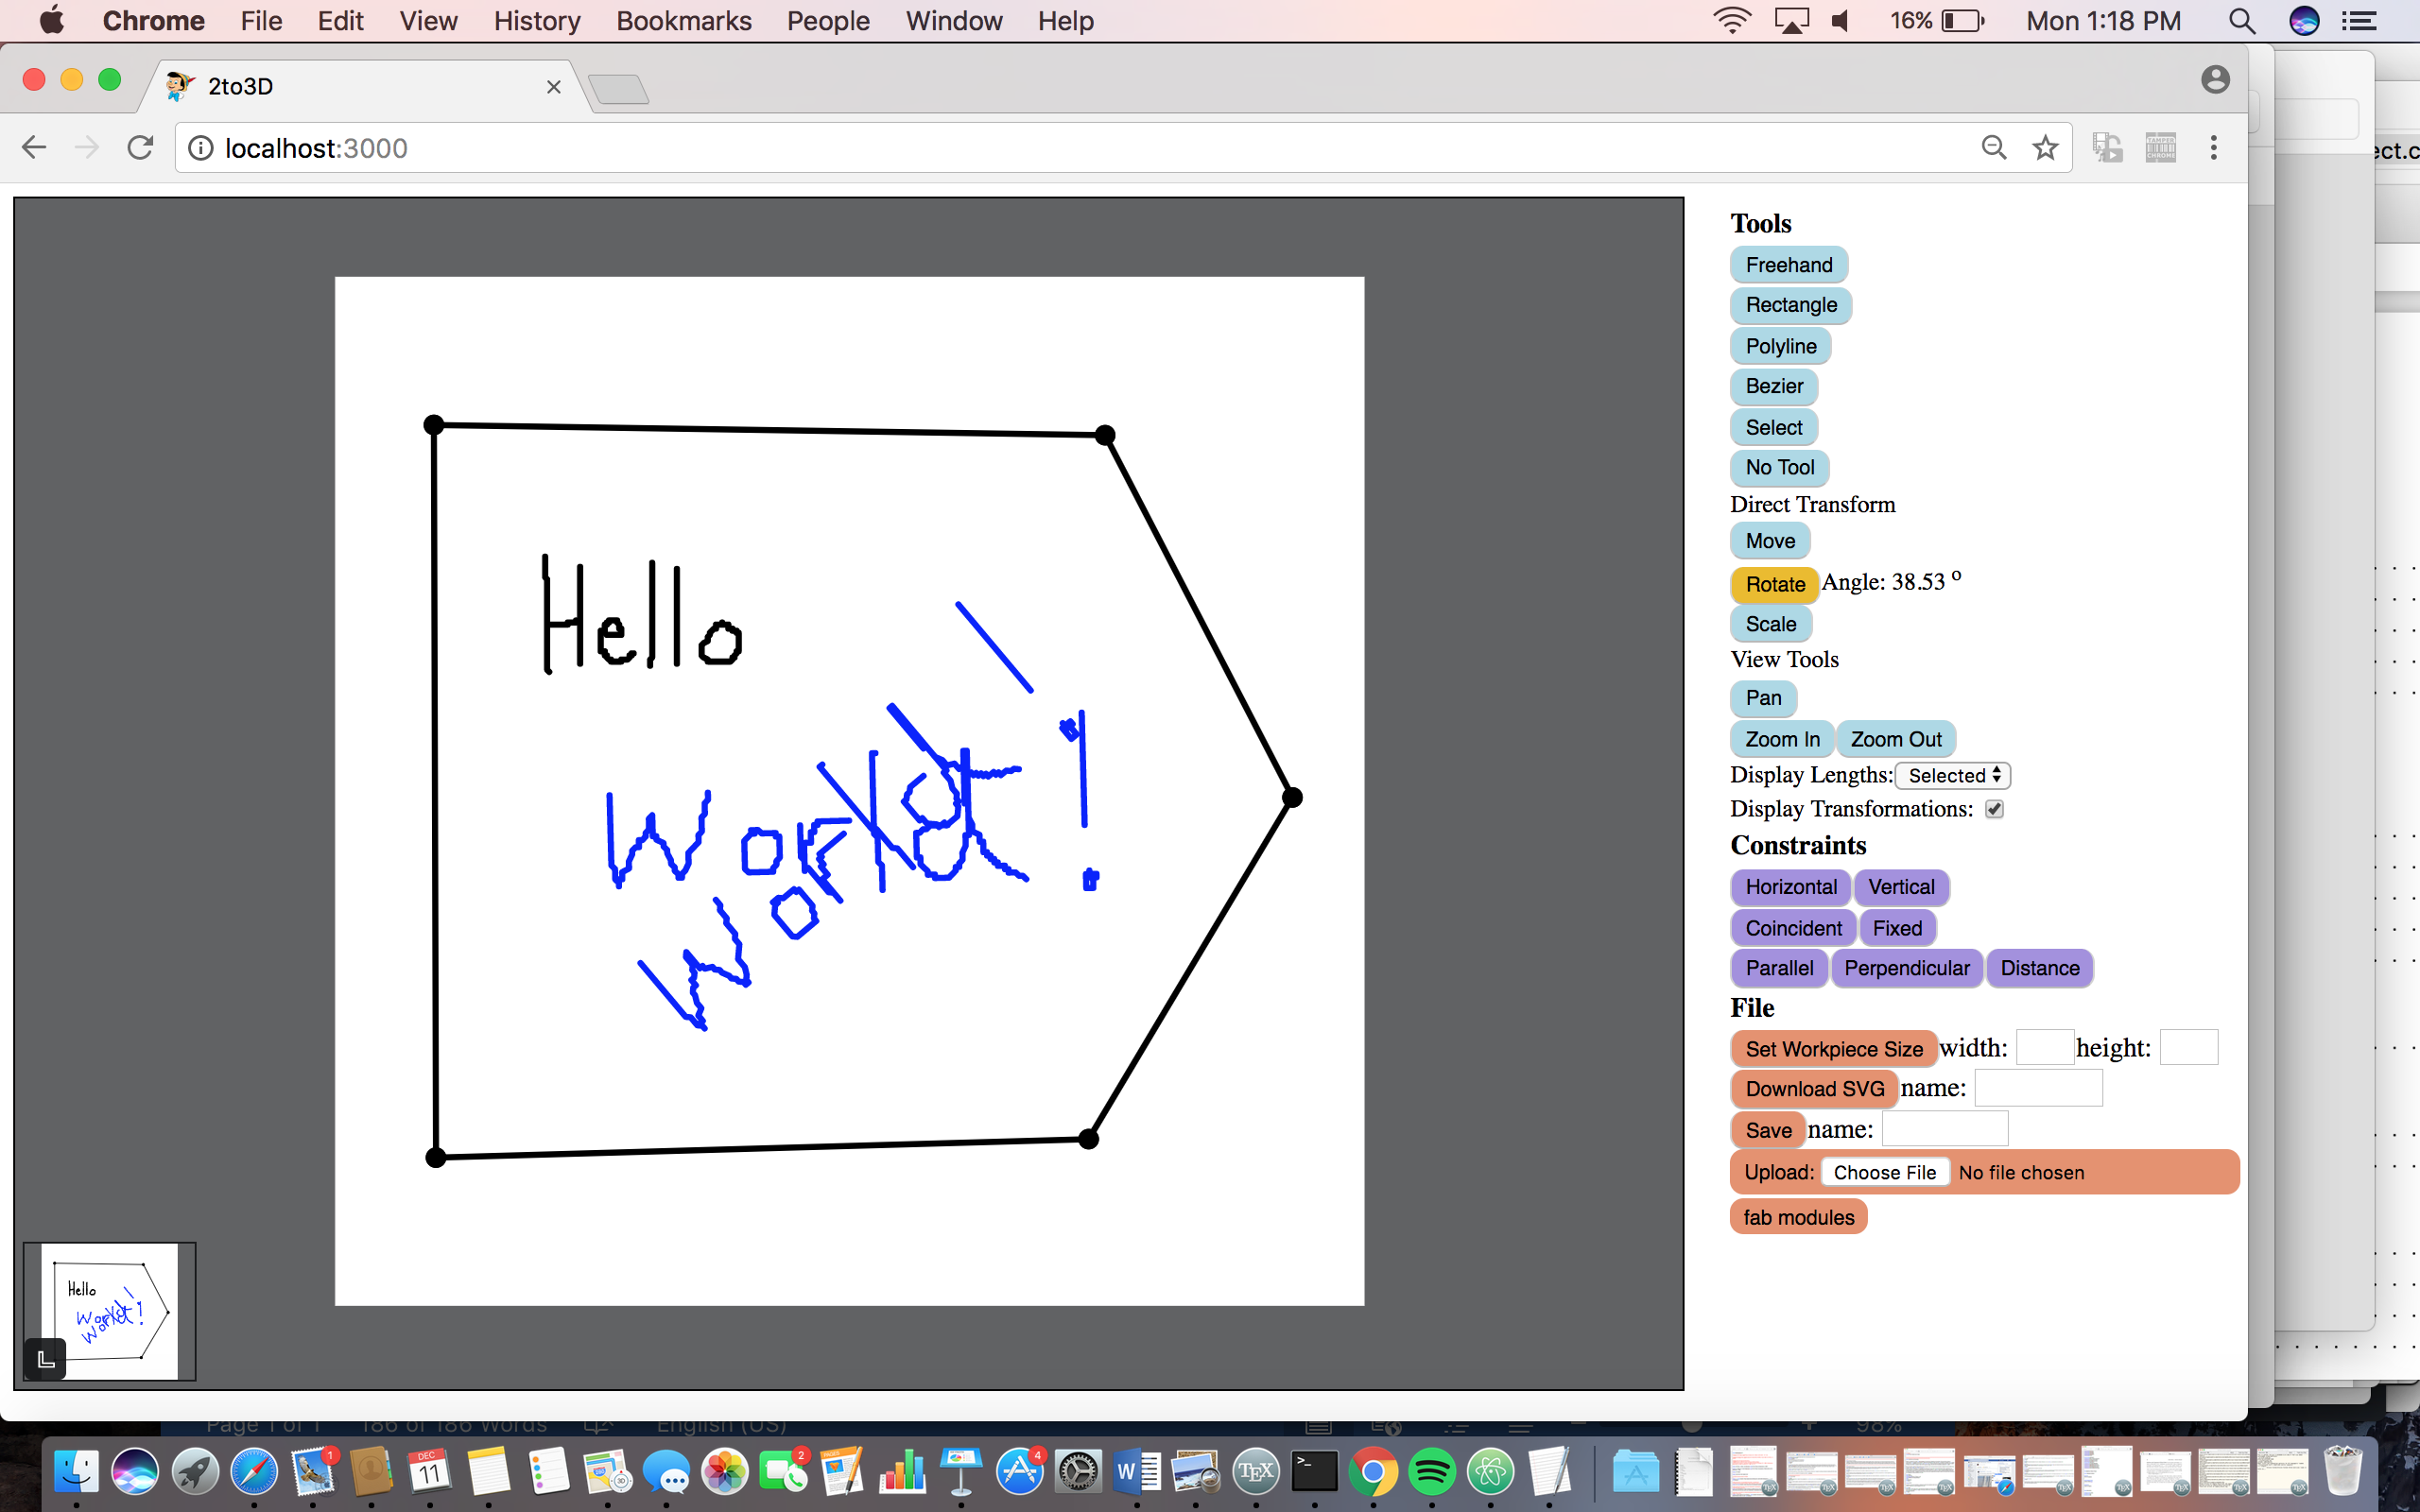
\includegraphics[width=\linewidth]{screenshot2.png}
  \caption{Screenshot of 2to3D program depicting rotation tool in action. Note the angle on display next to the highlighted tool in the right toolbox.}
  \label{fig:screenshot2}
\end{figure}

2to3D supports three shape primitives (line, bezier and freehand) which can be used to create more complex shapes. The program supports both linear and non-linear constraints but linear constraints are far more robust. The program also supports direct transformations - rotations, moves, and scales - that break constraints of transformed objects. This allows the user to make direct edits to drawing geometry that will exactly reflect user's intention. In addition to these three aspects which were detailed in Section 4, 2to3D also supports a myriad of other features. The drawing area allows zooming in/out and panning. The workpiece size is adjustable which facilitates creation of designs on any scale. SVG exports draw dimensions from workpiece size which simplifies the CAM process if the user decides to match drawing dimensions to laser cutter bed size. Hotkeys support swift and smooth workflows. Copy and paste capabilities allow users to quickly create redundant geometry. Geometry can be deleted to correct errors. And save and upload features allow users to continue work on unfinished projects or to share designs with others. Because the save feature relies on $JSON.stringify()$ the drawing objects must be rehydrated on upload. This means that shape primitives must have their prototype objects reset so they maintain methods. A full list of features can be found in Table~\ref{tab:capabilities}.

\begin{table}[H]
\centering
\caption{Capabilities of 2to3D.}
\label{tab:capabilities}
\begin{tabular}{|l|l|l|l|}
\hline
\multicolumn{2}{|l|}{{\ul \textbf{Drawing}}}                                                                                                                                                        & \multicolumn{2}{l|}{{\ul \textbf{Navigation}}}                                                                                                                                               \\
\multicolumn{2}{|l|}{\begin{tabular}[c]{@{}l@{}}Freehand\\ Rectangle\\ Polyline\\ Bezier\end{tabular}}                                                                                              & \multicolumn{2}{l|}{\begin{tabular}[c]{@{}l@{}}Pan\\ Zoom in/out\end{tabular}}                                                                                                               \\ \hline
\multicolumn{2}{|l|}{{\ul \textbf{Direct Transformations}}}                                                                                                                                         & \multicolumn{2}{l|}{{\ul \textbf{Display Options}}}                                                                                                                                          \\
\multicolumn{2}{|l|}{\begin{tabular}[c]{@{}l@{}}Move\\ Rotate\\ Scale\end{tabular}}                                                                                                                 & \multicolumn{2}{l|}{\begin{tabular}[c]{@{}l@{}}Lengths\\ Transformation values\end{tabular}}                                                                                                 \\ \hline
\multicolumn{2}{|l|}{{\ul \textbf{Constraints}}}                                                                                                                                                    & \multicolumn{2}{l|}{{\ul \textbf{Other}}}                                                                                                                                                    \\
\multicolumn{2}{|l|}{\begin{tabular}[c]{@{}l@{}}Horizontal (line)\\ Vertical (line)\\ Coincident (points)\\ Fixed (points)\\ Parallel (lines)\\ Perpendicular (lines)\\ Length (line)\end{tabular}} & \multicolumn{2}{l|}{\begin{tabular}[c]{@{}l@{}}Click and drag points\\ Download SVG\\ Save drawing\\ Upload drawing\\ Copy/Paste\\ Delete\\ Hotkeys\\ Workpiece size adjustable\end{tabular}} \\ \hline
\end{tabular}
\end{table}

\subsection*{Link to Video Demo and Program}
A demonstration of the program's features can be found at: \newline \underline{\url{https://www.youtube.com/watch?v=QDdJkAFzwLU}}. \newline

The program itself can be accessed while on Middlebury College's network at: \newline \underline{\url{basin.cs.middlebury.edu:3002}}.